\section{Systematic Uncertainties}

\begin{figure}[htbp]
	\centering
	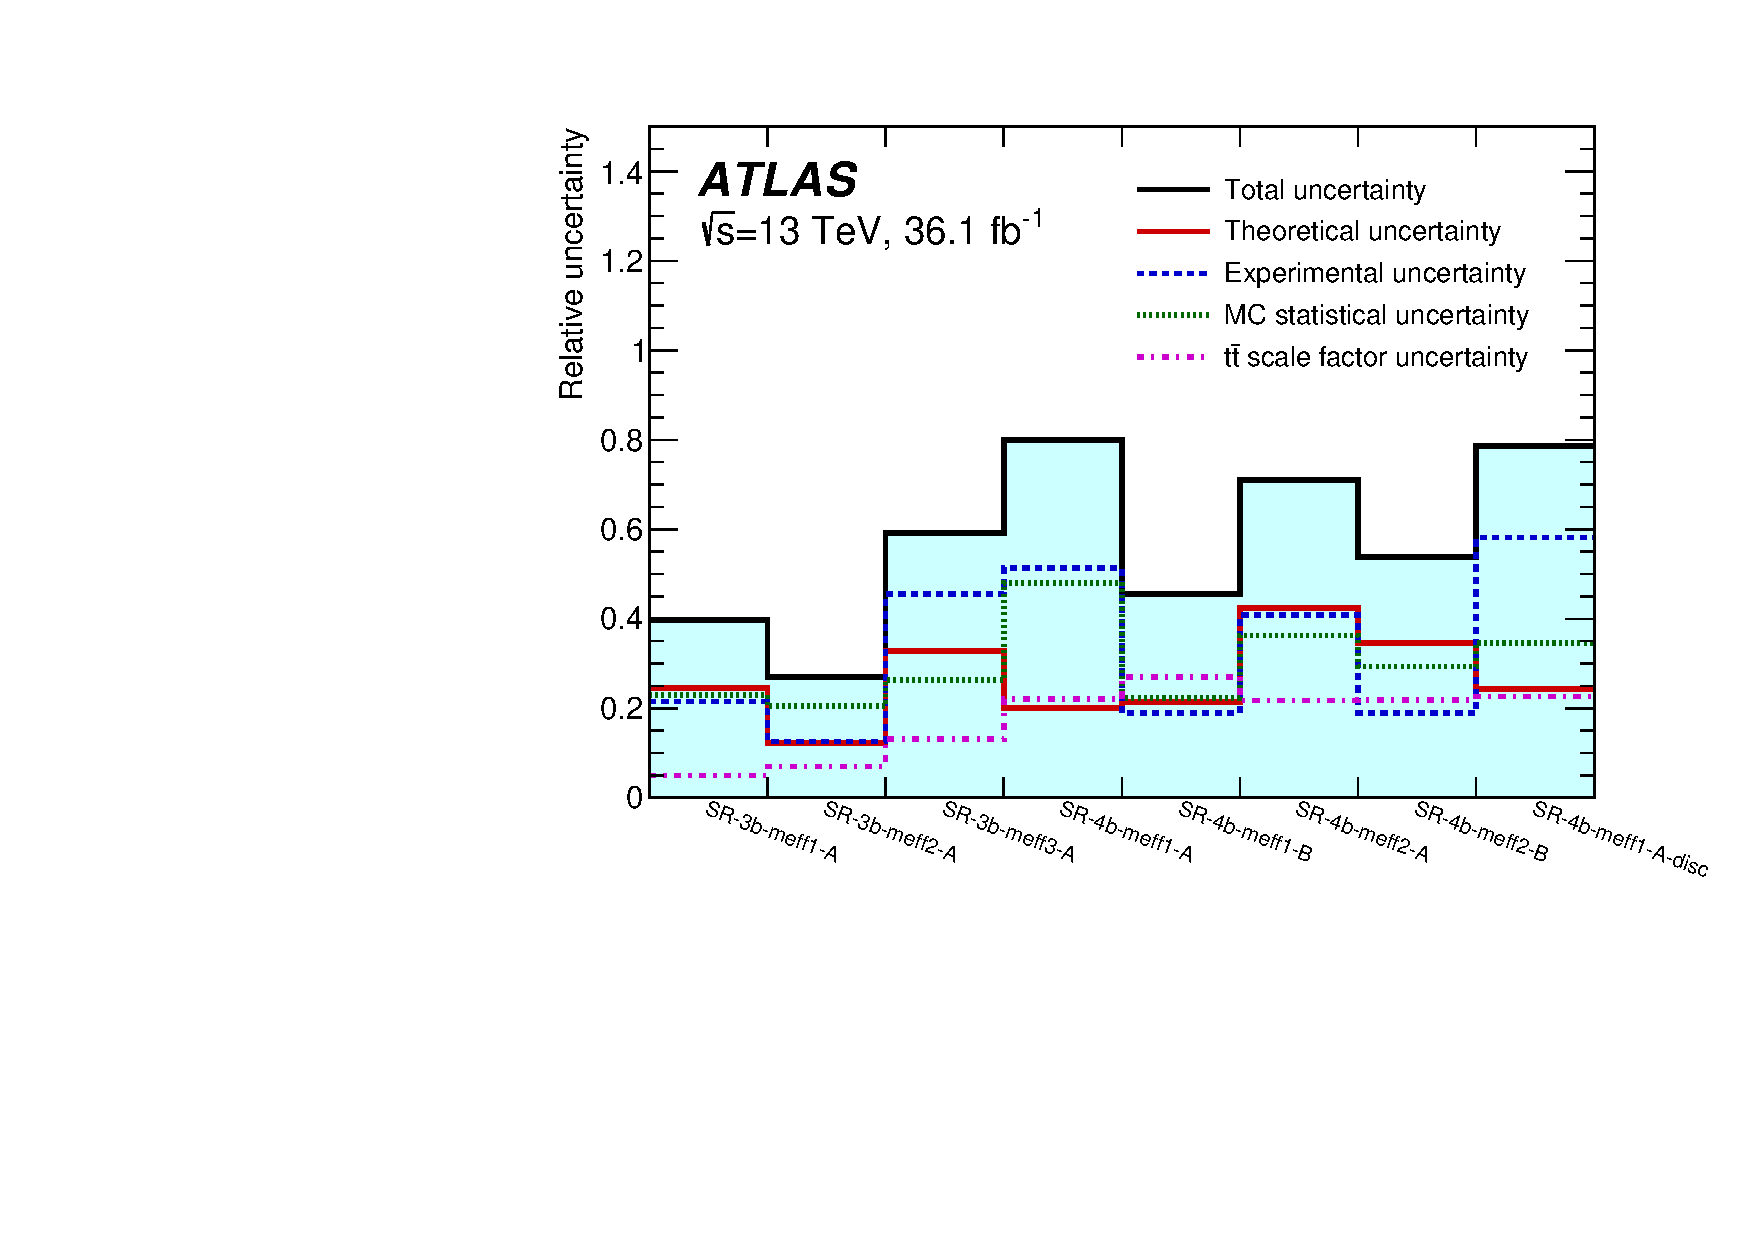
\includegraphics[width=0.85\textwidth]{figures/ewk_prod/etmiss_misc/High-MET-syst.pdf}
	\caption{Relative systematic uncertainties in the background estimate for the high-mass analysis. The individual uncertainties can be correlated, such that the total background uncertainty is not necessarily their sum in quadrature. 
	} 
	\label{fig:syst_etmiss}
\end{figure}

\section{Results}

\begin{figure}[htbp]
	\centering
	\includegraphics[width=0.9\textwidth]{figures/ewk_prod/etmiss_results/histpull_pulls_in_CR_qcdStrong}
	\caption{Event yields in control regions and related \ttbar\
          normalization factors after the background-only fit for
          %Inputs and results of the likelihood fit in the control
          %regions of
          the high-mass analysis. The upper panel shows 
		the observed number of events and the predicted background yield before the fit.
		All uncertainties described in Section \ref{sec:syst_high} are included in the uncertainty band. The background category $\ttbar+X$ includes $\ttbar W/Z$, $\ttbar H$, and $\ttbar \ttbar$ events.  
		The $\ttbar$ normalization is obtained from the fit
                and is displayed in the bottom panel.
	} 
	\label{fig:pullCR}
\end{figure}


\begin{figure}[htbp]
	\centering
	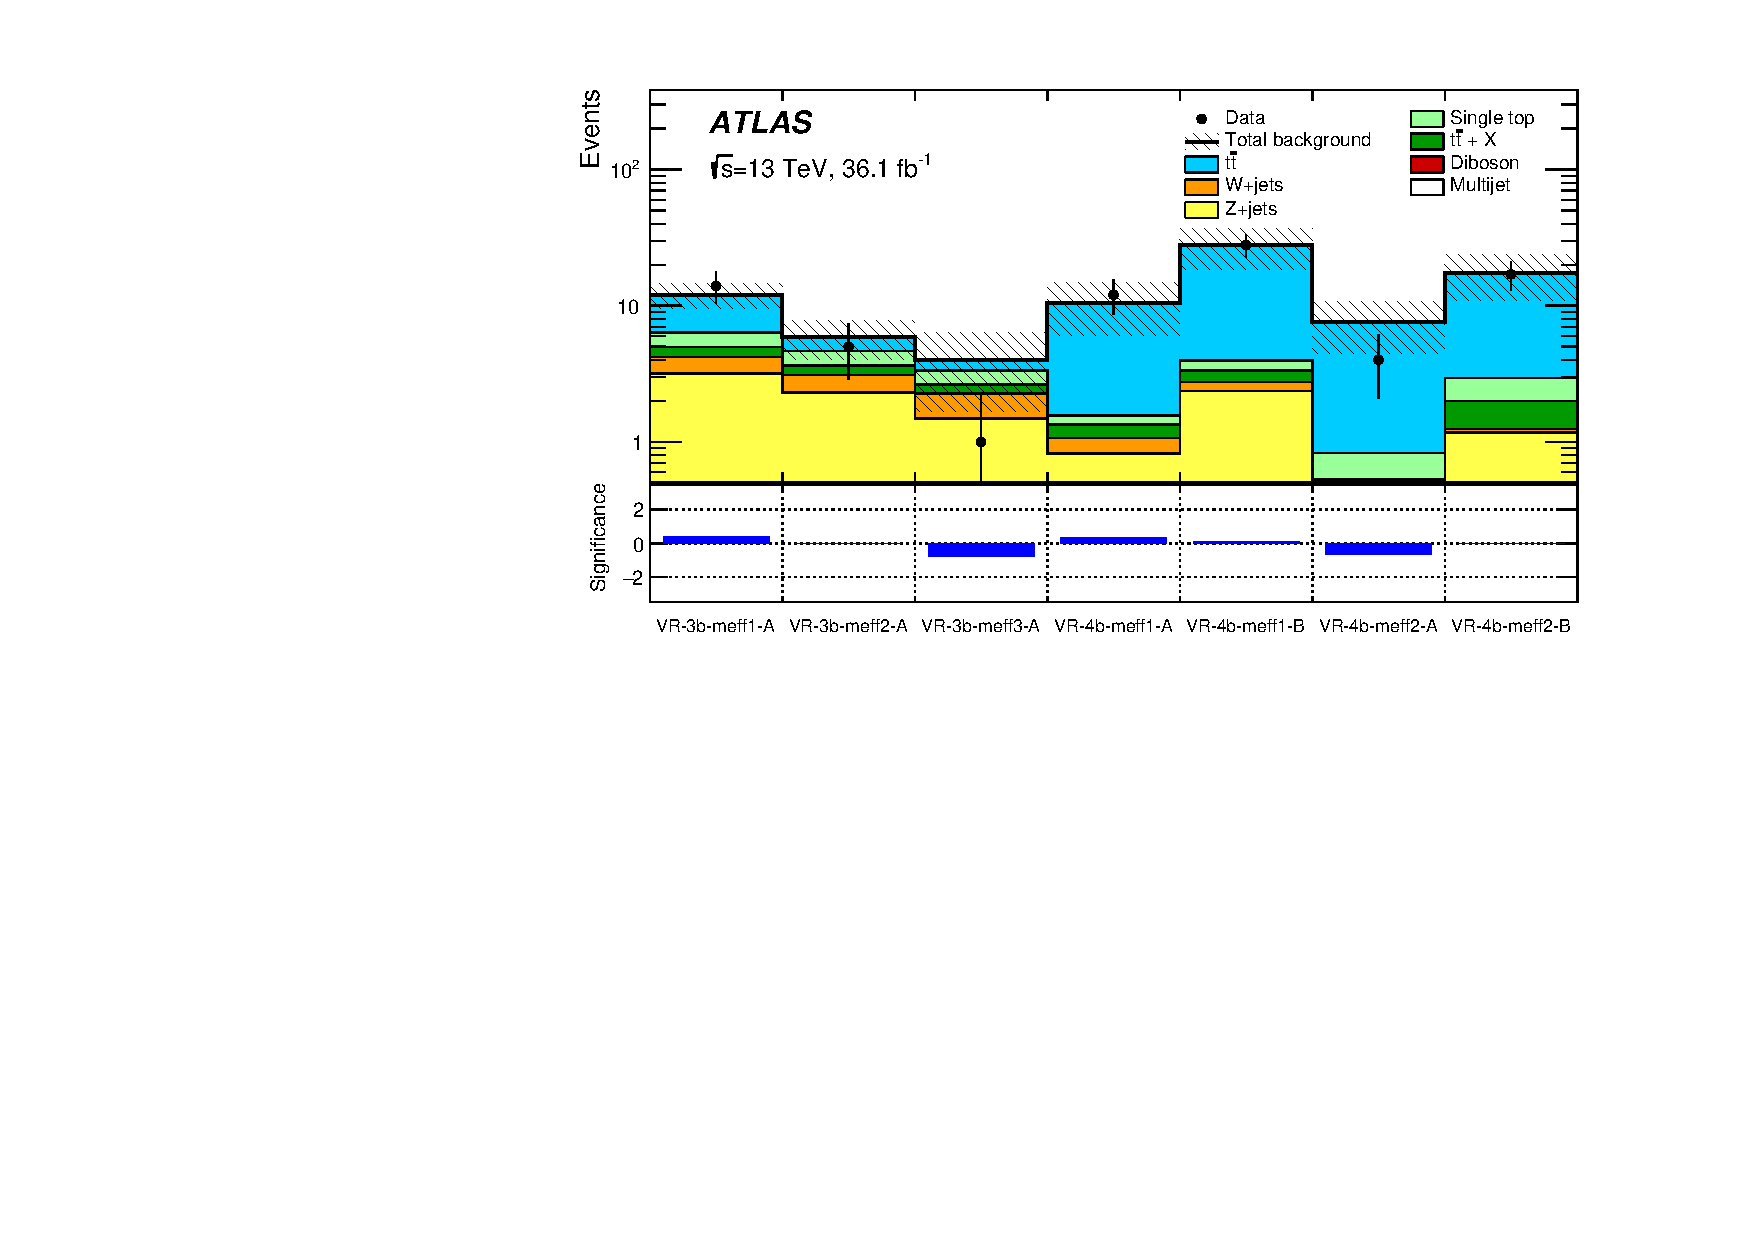
\includegraphics[width=0.9\textwidth]{figures/ewk_prod/etmiss_results/histpull_pulls_in_VR_qcdStrong}
	\caption{Results of the background-only fit extrapolated to the VRs of the high-mass analysis. The $\ttbar$ normalization 
		is obtained from the fit to the CRs shown in Figure~\ref{fig:pullCR}. The upper panel shows 
		the observed number of events and the predicted background yield. The bottom panel shows the significance of any disagreement between the data and the background model~\cite{Choudalakis2012}.
		All uncertainties  defined in Section~\ref{sec:syst_high} are included in the 
		uncertainty band. The background category $\ttbar+X$ includes $\ttbar W/Z$, 
		$\ttbar H$, and $\ttbar \ttbar$ events. }
	\label{fig:pullVR}
\end{figure}

\begin{figure}[htbp]
	\centering
	% \subfigure[]{\includegraphics[width=0.65\textwidth]{figures/etmiss_results/histpull_pulls_in_CR_qcdStrong}\label{fig:pullCR}}\\
	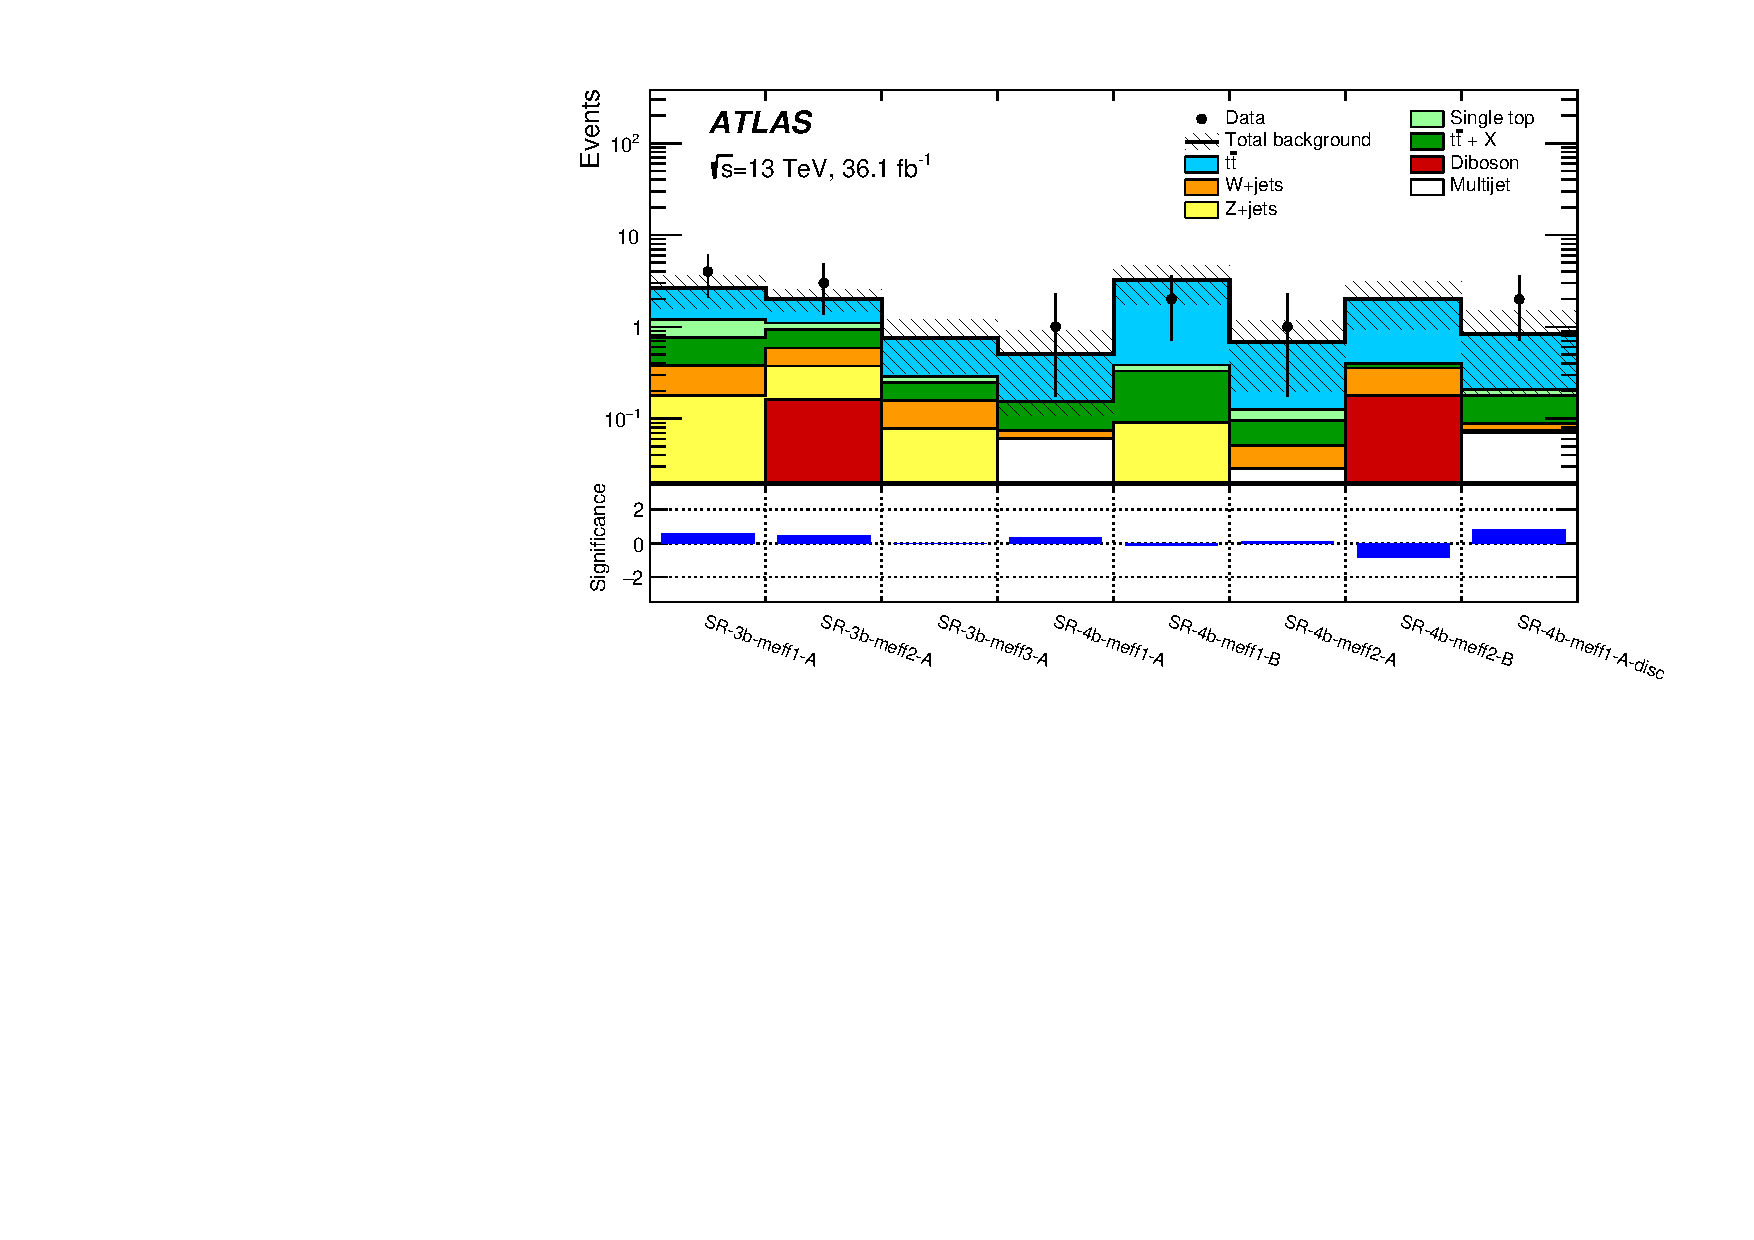
\includegraphics[width=0.9\textwidth]{figures/ewk_prod/etmiss_results/histpull_pulls_in_SR_qcdStrong}
	\caption{Results of the background only fit extrapolated to the SRs of the high-mass analysis. The $\ttbar$ normalization
                is obtained from the fit to the CRs shown in Figure~\ref{fig:pullCR}. The data in the  SRs are 
	not included in the fit.  The upper panel shows the observed number of events and the predicted background 
	yield.  The bottom panel shows the significance of any disagreement between the data and the background model~\cite{Choudalakis2012}. All uncertainties  defined in Section~\ref{sec:syst_high} are included in the uncertainty band. The background
	category $\ttbar+X$ includes $\ttbar W/Z$, $\ttbar H$, and $\ttbar \ttbar$ events.} 
	\label{fig:pullSR}
\end{figure}

\begin{table}
%\resizebox{1.\textwidth}{!}{
\renewcommand{\arraystretch}{1.1}
\begin{tabular}{l|c|c|c|c}
\toprule
SR name & SR-3b-meff1-A & SR-3b-meff2-A & SR-3b-meff3-A & SR-4b-meff1-A \\
\hline
$N_{\mathrm{obs}}$ & 4 & 3 & 0 & 1 \\
\hline
Total background & 2.6 $\pm$ 1.0 & 2.0 $\pm$ 0.5 & 0.8 $\pm$ 0.5 & 0.5 $\pm$ 0.4  \\
Fitted \ttbar & 1.4 $\pm$ 0.8 & 0.89 $\pm$ 0.32 & 0.5 $\pm$ 0.4 & 0.35 $\pm$ 0.33 \\

Single top & 0.43 $\pm$ 0.29 & 0.17 $\pm$ 0.14 & 0.040 $\pm$ 0.017 & $<$ 0.01 \\
$\ttbar+X$ & 0.39 $\pm$ 0.16 & 0.34 $\pm$ 0.14 & 0.09 $\pm$ 0.04 & 0.08 $\pm$ 0.06  \\
$Z$+jets & 0.18 $\pm$ 0.14 & 0.21 $\pm$ 0.16 & 0.07 $\pm$ 0.20 & $<$ 0.01 \\
$W$+jets & 0.20 $\pm$ 0.06 & 0.21 $\pm$ 0.09 & 0.08 $\pm$ 0.06 & 0.013 $\pm$ 0.009  \\
Diboson & $<$ 0.01 & 0.16 $\pm$ 0.11 & $<$ 0.01 & $<$ 0.01 \\
Multijet & $<$ 0.01 & 0.004 $\pm$ 0.005 & 0.004 $\pm$ 0.006 & 0.06 $\pm$ 0.05 \\
\hline
MC-only background & 2.5 $\pm$ 1.0 & 2.0 $\pm$ 0.5 & 0.6 $\pm$ 0.4 & 0.43 $\pm$ 0.31 \\
\bottomrule
\end{tabular}

\vspace{0.4cm}

\begin{tabular}{l|c|c|c|c}
\toprule
SR name & SR-4b-meff1-B & SR-4b-meff2-A & SR-4b-meff2-B & SR-4b-meff1-A-disc\\
\hline
$N_{\mathrm{obs}}$ & 2 & 1 & 0 & 2\\
\hline
Total background &  3.2 $\pm$ 1.5 & 0.7 $\pm$ 0.5 & 2.0 $\pm$ 1.1 & 0.8 $\pm$ 0.7\\
Fitted \ttbar &  2.8 $\pm$ 1.5 & 0.6 $\pm$ 0.5 & 1.6 $\pm$ 1.0 & 0.6 $\pm$ 0.6\\
Single top &  0.06 $\pm$ 0.13 & 0.030 $\pm$ 0.019 & $<$ 0.01 & 0.030 $\pm$ 0.019\\
$\ttbar+X$ & 0.24 $\pm$ 0.10 & 0.045 $\pm$ 0.025 & 0.039 $\pm$ 0.033 & 0.09 $\pm$ 0.06\\
$Z$+jets &  0.09 $\pm$ 0.04 & $<$ 0.01 & $<$ 0.01 & 0.004 $\pm$ 0.011\\
$W$+jets & $<$ 0.01 & 0.022 $\pm$ 0.027 & 0.18 $\pm$ 0.10 & 0.013 $\pm$ 0.008\\
Diboson &  $<$ 0.01 & $<$ 0.01 & 0.17 $\pm$ 0.08 & $<$ 0.01\\
Multijet &  0.0027 $\pm$ 0.0021 & 0.03 $\pm$ 0.04 & 0.007 $\pm$ 0.012 & 0.07 $\pm$ 0.05\\
\hline
MC-only background & 2.6 $\pm$ 0.9 & 0.43 $\pm$ 0.27 & 1.3 $\pm$ 0.6 & 0.7 $\pm$ 0.5\\
\bottomrule
\end{tabular}
%} 
\caption{Results of the background-only fit extrapolated to the SRs of the high-mass analysis, for the total background prediction and breakdown of the main background sources. 
	The uncertainties shown include all systematic uncertainties. The data in the SRs are not included in the fit. 
	The background category $\ttbar+X$ includes $\ttbar W/Z$, $\ttbar H$, and $\ttbar \ttbar$ events.
	The row ``MC-only background'' provides the total background prediction when the
	$\ttbar$ normalization is obtained from a theoretical
	calculation~\cite{Czakon:2011xx}.}
\label{tab:yieldsSR}
\end{table}




\clearpage

\section{Interpretation}
\label{sec:ewk:interp}

\begin{table}
\begin{center}
\begin{tabular}{
      lr
      S[table-format=4.1(1)]
      S[table-format=1.1(2)]
      S[table-format=2.1(1)]
      cc
      }
\toprule
{ Signal channel}           &   $N_\mathrm{obs}$ & \multicolumn{1}{c}{$N_\mathrm{pred}$}       & \multicolumn{1}{c}{$\sigma^\mathrm{95}_\mathrm{vis}$ [fb]}  &  $S_\mathrm{obs}^\mathrm{95}$  & $S_\mathrm{exp}^\mathrm{95}$ & $p_0$ (Z)  \\
\midrule
high-SR-4b-meff1-A-disc   &    2 &     0.8 \pm 0.7  & 0.15 &   5.5 & ${ 4.2 }^{ +1.3 }_{ -0.4 }$  &  0.15$~$(1.02) \\%
high-SR-3b-meff3-A        &    0 &     0.8 \pm 0.5  & 0.08 &   3.0 & ${ 3.1 }^{ +1.2 }_{ -0.1 }$  &  0.50$~$(0.00) \\%
low-SR-MET0-meff440       & 1063 &    1100 \pm 25   & 2.3  &  56   & ${ 79 }^{ +31 }_{ -23 }$     &  0.50$~$(0.00) \\%
low-SR-MET150-meff440     &   17 &      12 \pm 8    & 0.90 &  22   & ${ 19 }^{ +5 }_{ -4 }$       &  0.21$~$(0.80) \\%
\bottomrule
\end{tabular}
\end{center}
\caption[Model independent upper limits]{For each discovery region, the number of observed events ($N_\mathrm{obs}$), the number of predicted events ($N_\mathrm{pred}$), and 95\% CL upper limits on the visible cross-section ($\sigma^\mathrm{95}_\mathrm{vis}$) and on the number of signal events ($S_\mathrm{obs}^\mathrm{95}$ ) are shown.  The fifth column ($S_\mathrm{exp}^\mathrm{95}$) shows the 95\% CL upper limit on the number of signal events given the expected number (and $\pm 1\sigma$ excursions of the expectation) of background events. The last column indicates the discovery $p$-value ($p(s~=~0)$) in significance units. The $p$-values are capped at 0.5. Results are obtained with $20\,000$ pseudoexperiments.}
\label{tab:UL_toys}
\end{table}


\begin{figure}[htbp]
	\centering
	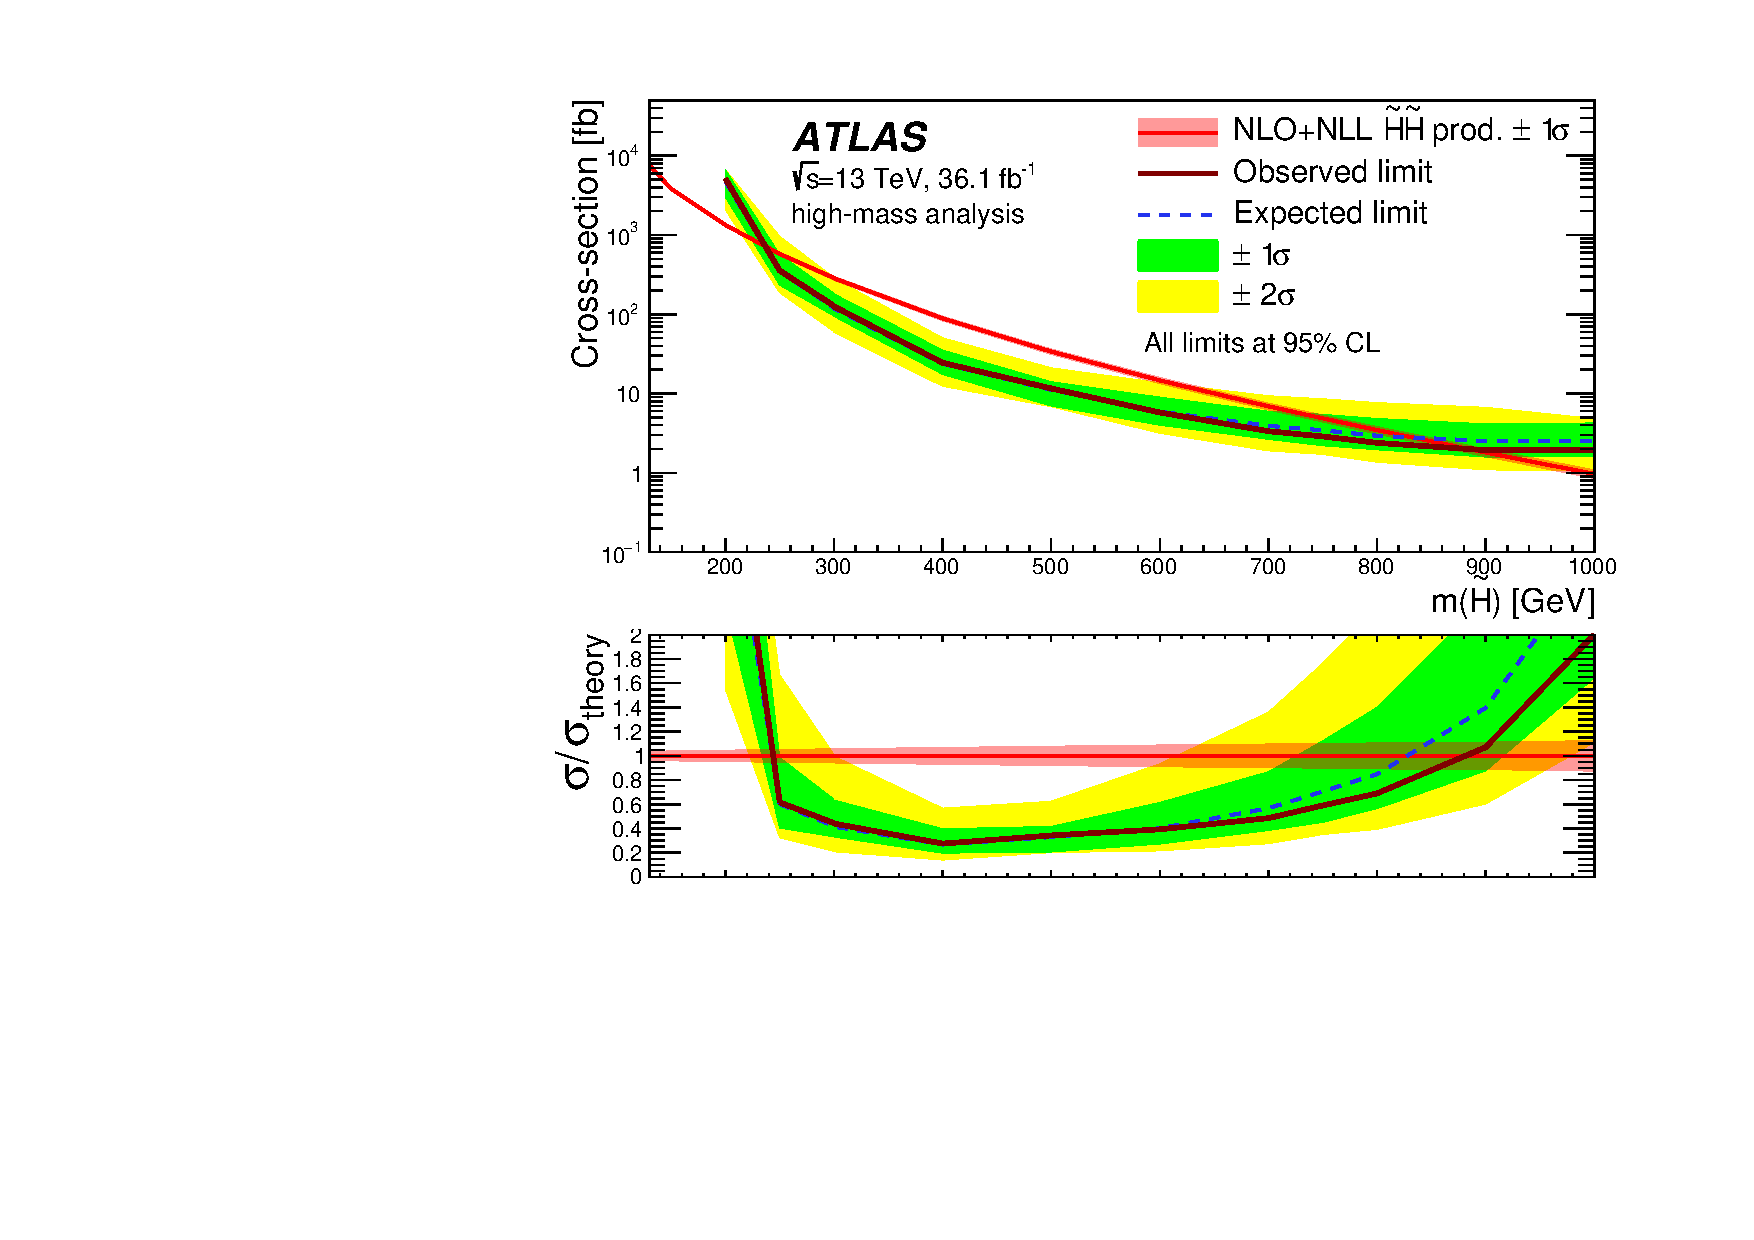
\includegraphics[width=0.8\textwidth]{figures/ewk_prod/interpretation/limit_HM}
	\caption{The observed (solid black) vs expected (dashed black) 95\% upper limits on the total pair production cross section for degenerate higgsinos as a function of \mhino\ for the high-mass search. The 1 and 2$\sigma$ uncertainty bands are shown as green and yellow, respectively. Only the high-mass analysis results are used in this figure. The theory cross section is shown in the red curve. The bottom panel shows the ratio of the observed and expected limits with the theory cross section.} 
	\label{fig:exclusion_high}
\end{figure}

\begin{figure}[htbp]
	\centering
	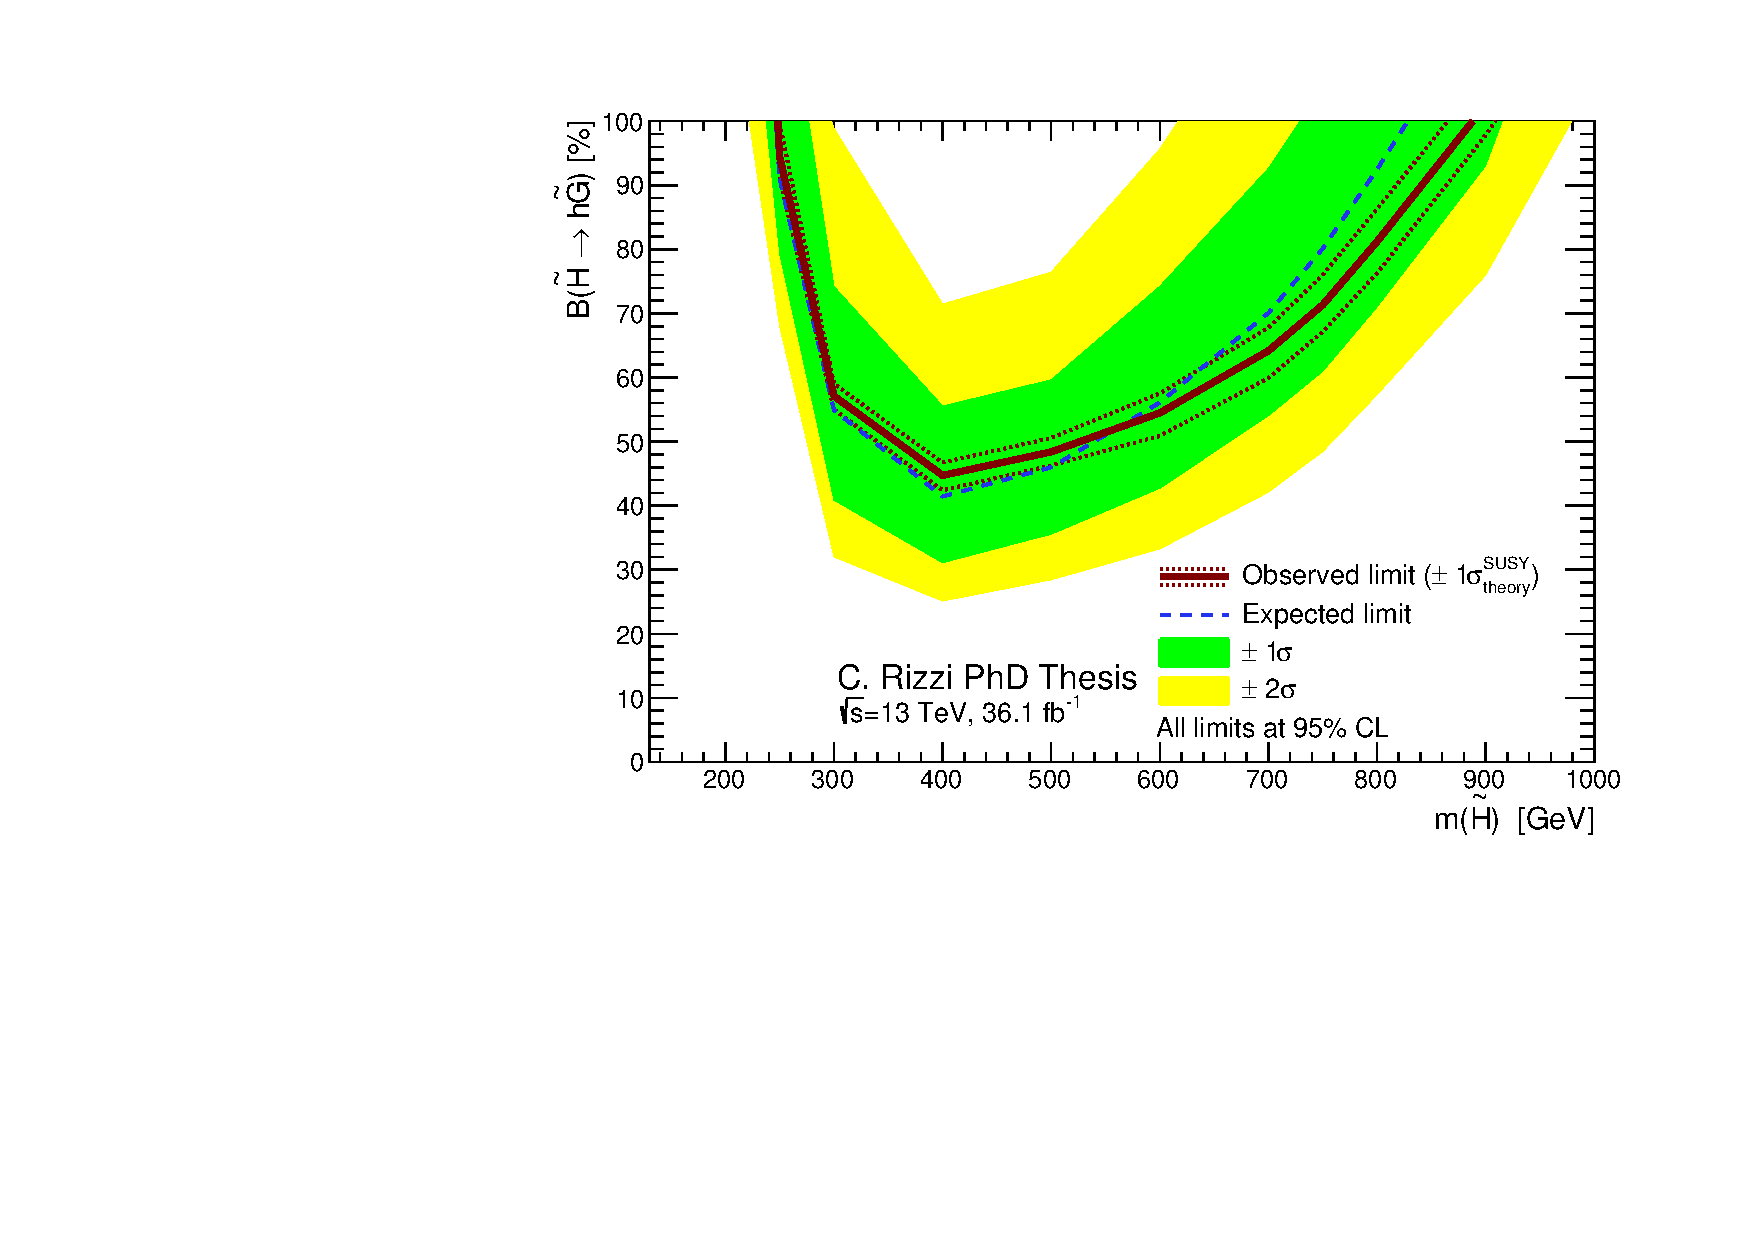
\includegraphics[width=0.8\textwidth]{figures/ewk_prod/interpretation/br_limit_HM.pdf}
	\caption{BR limit} 
	\label{fig:exclusion_high}
\end{figure}



